% LaTeX template for creating an MNRAS paper
%
% v3.2 released 20 July 2023
% (version numbers match those of mnras.cls)
%
% Copyright (C) Royal Astronomical Society 2015
% Authors:
% Keith T. Smith (Royal Astronomical Society)

%%%%%%%%%%%%%%%%%%%%%%%%%%%%%%%%%%%%%%%%%%%%%%%%%%%%%%%%%%%%%%%%%%%%%%%%%%%%%%%%%%%%%%%%%%%%%%%%%%%%
% Basic setup. Most papers should leave these options alone.
\documentclass[fleqn,usenatbib]{mnras}

% MNRAS is set in Times font. If you don't have this installed (most LaTeX
% installations will be fine) or prefer the old Computer Modern fonts, comment
% out the following line
\usepackage{newtxtext,newtxmath}
% Depending on your LaTeX fonts installation, you might get better results with one of these:
%\usepackage{mathptmx}
%\usepackage{txfonts}

% Use vector fonts, so it zooms properly in on-screen viewing software
% Don't change these lines unless you know what you are doing
\usepackage[T1]{fontenc}

% Allow "Thomas van Noord" and "Simon de Laguarde" and alike to be sorted by "N" and "L" etc. in the bibliography.
% Write the name in the bibliography as "\VAN{Noord}{Van}{van} Noord, Thomas"
\DeclareRobustCommand{\VAN}[3]{#2}
\let\VANthebibliography\thebibliography
\def\thebibliography{\DeclareRobustCommand{\VAN}[3]{##3}\VANthebibliography}


%%%%% AUTHORS - PLACE YOUR OWN PACKAGES HERE %%%%%

% Only include extra packages if you really need them. Avoid using amssymb if newtxmath is enabled, as these packages can cause conflicts. newtxmatch covers the same math symbols while producing a consistent Times New Roman font. Common packages are:
\usepackage{graphicx}	
\usepackage{amsmath}	
\usepackage{physics}
\usepackage{enumitem}
\usepackage{anyfontsize}
\usepackage{placeins}
\usepackage{cleveref}


%%%%%%%%%%%%%%%%%%%%%%%%%%%%%%%%%%%%%%%%%%%%%%%%%%%%%%%%%%%%%%%%%%%%%%%%%%%%%%%%%%%%%%%%%%%%%%%%%%%%

%%%%% AUTHORS - PLACE YOUR OWN COMMANDS HERE %%%%%

% Please keep new commands to a minimum, and use \newcommand not \def to avoid
% overwriting existing commands. Example:
%\newcommand{\pcm}{\,cm$^{-2}$}	% per cm-squared

\graphicspath{{images/}}
%\raggedbottom               %This will let the height of the textblock vary from page to page. 

% Command to use placeins with \subsection
\makeatletter
\AtBeginDocument{%
  \expandafter\renewcommand\expandafter\subsection\expandafter
    {\expandafter\@fb@secFB\subsection}%
  \newcommand\@fb@secFB{\FloatBarrier
    \gdef\@fb@afterHHook{\@fb@topbarrier \gdef\@fb@afterHHook{}}}%
  \g@addto@macro\@afterheading{\@fb@afterHHook}%
  \gdef\@fb@afterHHook{}%
}
\makeatother

%%%%%%%%%%%%%%%%%%%%%%%%%%%%%%%%%%%%%%%%%%%%%%%%%%%%%%%%%%%%%%%%%%%%%%%%%%%%%%%%%%%%%%%%%%%%%%%%%%%%


%%%%%%%%%%%%%%%%%%% TITLE PAGE %%%%%%%%%%%%%%%%%%%%%%%%%%%%%%%%%%%%%%%%%%%%%%%%%%%%%%%%%%%%%%%%%%%%%

% Title of the paper, and the short title which is used in the headers.
% Keep the title short and informative.
\title[]{Study of the star formation rate bimodality in SDSS galaxies at low redshift}

% The list of authors, and the short list which is used in the headers.
% If you need two or more lines of authors, add an extra line using \newauthor
\author[Marco Bianchi]{
Marco Bianchi
\\
% List of institutions
University of Milano-Bicocca, Physics Department, Astrophysics and Space Physics master degree\\
Laboratory of Data Analysis 2023-2024, group 5: M. Bellotti, M. Bianchi, L. Carbone, and F. Leto Di Priolo
}

% Enter the current year, for the copyright statements etc.
\pubyear{2024}

% Don't change these lines
\begin{document}
\label{firstpage}
\pagerange{\pageref{firstpage}--\pageref{lastpage}}
\maketitle

% Abstract of the paper
\begin{abstract}
Galaxies at low redshift ($z<0.08$ for the data used here) display a bimodality in their specific star formation rate (sSFR). This phenomenon is related to several factors, including (1) the accretion processes that drive galaxy growth, (2) the feedback processes that eject gas from galaxies, and (3) the interactions between galaxies and their surrounding environment. These processes are strongly influenced by key physical properties of galaxies, such as gas mass, stellar mass, and age. Therefore, it is possible to build models that describe the time evolution of sSFR based on these simple quantities. \\
We developed two very simple analytical models, based on strong assumptions, and applied them to a subset of the Sloan Digital Sky Survey (SDSS) dataset. Our findings indicate that young, actively star-forming galaxies can be described by an open-box model, while old, passive galaxies are better represented by a closed-box model, which does not exchange gas with the surrounding halo. We also relaxed some assumptions, such as redshift-independent gas accretion, by numerically integrating the differential equation of the open-box model over infinitesimal time steps, obtaining similar results.
\smallskip
\end{abstract} 
%%%%%%%%%%%%%%%%%%%%%%%%%%%%%%%%%%%%%%%%%%%%%%%%%%%%%%%%%%%%%%%%%%%%%%%%%%%%%%%%%%%%%%%%%%%%%%%%%%%%




%%%%%%%%%%%%%%%%% BODY OF PAPER %%%%%%%%%%%%%%%%%%%%%%%%%%%%%%%%%%%%%%%%%%%%%%%%%%%%%%%%%%%%%%%%%%%%

\section{Introduction}\label{sec:introduction}
Galaxies are the fundamental building blocks of the universe at cosmological scales. Therefore, understanding how they form, evolve over time, and interact, creating complex structures, is crucial for advancing our knowledge about the universe and its history. However, capturing the extreme diversity of galaxies in a mathematical model is a very challenging task.

In this context, it is well known \citep[e.g.,][]{Kauffmann_2003} that two main populations can be identified in the plane of \textbf{specific star formation rate} (sSFR) versus \textbf{stellar mass} ($M_{\text{star}}$): one of young, actively star-forming galaxies (the \textit{main sequence}) and the other of old, mostly passive galaxies, as shown in Fig.~\ref{fig:mass_sSFR}. For this reason, a model relating sSFR and $M_{\text{star}}$ should have at least two regimes, with a sharp transition past some threshold. In this work, we investigate the processes that either stimulate or quench the formation of new stars within galaxies at low redshift, and we try to develop simple mathematical models to test our assumptions.

The raw material for star formation is gas, which, under appropriate conditions, can collapse and form virialized objects. The amount of gas within a galaxy is not constant and is subject to a myriad of processes that depend on the main physical properties of the galaxy, such as age and mass. Therefore, we expect sSFR to drop whenever the consumed gas is no longer replaced by new gas, coming either from stars (winds, supernovae) or from outside the galaxy. 

In particular, gas inflow is strongly related to the properties of the dark matter halo that hosts the galaxy. This halo accretes matter from the intergalactic medium, a fraction $f_{\text{gas}}$ of which is gas, typically at very high temperature. Such hot gas has very strong pressure support that prevents it from accreting onto the galaxy. Therefore, the gas must cool down before it can infall, i.e., the condition $\tau_{\text{cooling}} < \tau_{\text{free-fall}}$ is required. This condition can be translated into a requirement on \textbf{halo mass} (for details, see chapter 8.4 of \citet{galaxy_formation_and_evolution_2010}). We make the following conservative assumption to have effective cooling:
\begin{equation}
    M_{\text{halo}} \in \left( M_{\text{halo,min}}=10^9 M_\odot \, , \, M_{\text{halo,max}}=10^{11.6} M_\odot \right),
	\label{eq:halo_mass_minmax}
\end{equation}

On the other hand, gas can also be expelled from the galaxy due to various processes, such as supernovae, AGN emission, and ram-pressure stripping. For simplicity, we will assume that Type IIA supernovae are the only source of gas outflow, given their dominant role. However, not all gas expelled by supernovae gains enough energy to escape the galaxy; indeed, some of it returns to the gas reservoir of the galaxy, increasing its metallicity. 

In Sec.~\ref{sec:methods}, we will present the dataset and the techniques we used, then, in Sec.~\ref{sec:results}, we will develop the concepts introduced here in a more mathematical way and present our results. Finally, in Sec.~\ref{sec:discussion}, we will discuss our results and draw conclusions from them.

\begin{figure}\centering
	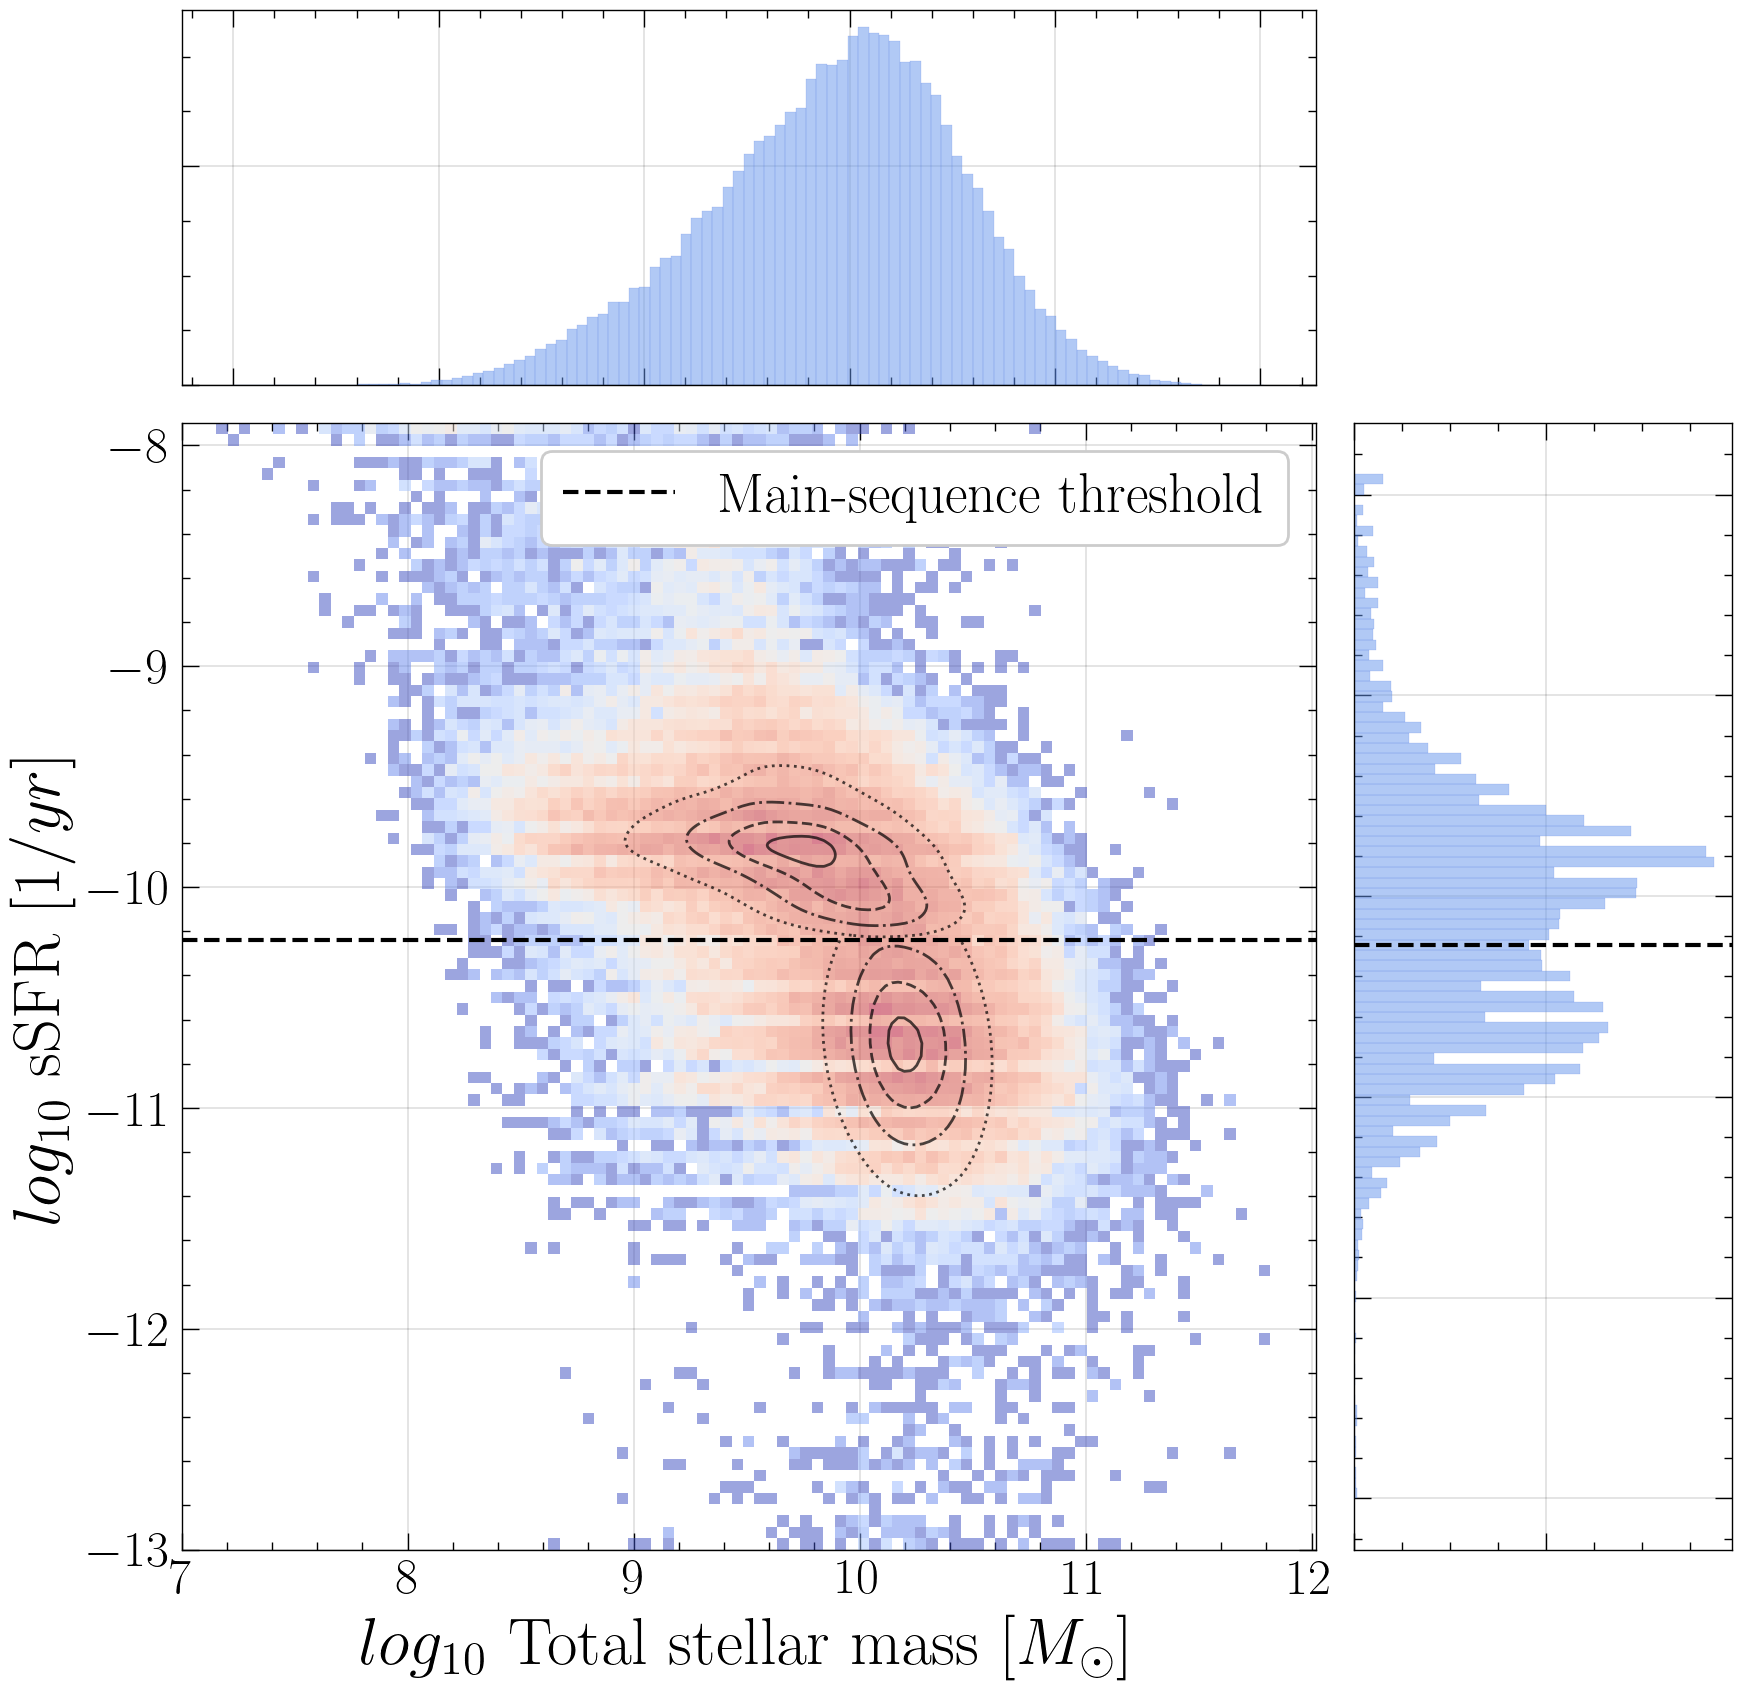
\includegraphics[width=0.84\columnwidth]{mass_sSFR.png}
    \caption{The main panel shows a 2D histogram of sSFR versus $M_{\text{star}}$ for our dataset. The side panels display the marginal distributions of the two axes. The black dashed line indicates the value where the sSFR distribution has a local minimum, which is used to separate the main sequence from passive galaxies. The 25, 50, 75, and 95\% contours of both populations are shown.}
    \label{fig:mass_sSFR}
\end{figure}
%%%%%%%%%%%%%%%%%%%%%%%%%%%%%%%%%%%%%%%%%%%%%%%%%%



\section{Methods}\label{sec:methods}
This work is based on a subset of the \textbf{Sloan Digital Sky Survey} (SDSS) dataset. In particular, we study $92483$ galaxies with redshift $< 0.08$ ($z_{\text{mean}} \simeq 0.054$), for which we have five-band photometric data. This data may seem too sparse to obtain a valuable estimate of the SFR, but we have been able to achieve this by employing a powerful library called \textbf{CIGALE} (Code Investigating GALaxy Emission). It generates a grid of model parameters and fits the photometric data with each model, selecting the best one through a bayesian approach based on likelihood maximization. The way in which CIGALE builds its models is quite sophisticated, as it takes into account a many factors, such as:
\begin{itemize}[left=6pt]
    \item \textbf{Star formation history (SFH):} describes how the SFR changes over time.
    \item \textbf{Initial mass function (IMF):} describes the mass distribution of newly-formed stars.
    \item \textbf{Stellar population synthesis (SPS):} describes the spectrum emitted by a certain stellar population at a given time. This population is formed according to a SFH, an IMF, and an initial metallicity. It takes into account how stars evolve over time, as a function of mass and metallicity.
    \item \textbf{Dust attenuation:} describes how the light emitted by stars is absorbed and re-emitted by galactic dust.
    \item \textbf{Nebular emission:} describes the light emitted by ionized gas regions within the galaxy.
\end{itemize}
We choose (1) to model SFH with a double exponential, (2) to employ the IMF by \citet{Chabrier_2003}, (3) to model SPS according to \citet{Bruzual_2003}, (4) to model dust attenuation with \citet{Calzetti_2000} and \citet{Leitherer_2002} formulae, and (5) to take into account nebular emission. This is just a brief description of how CIGALE works, we suggest checking the original paper \citep{Boquien_2019} for the details.

Besides SFR, CIGALE provides a series of valuable estimates of galactic quantities, such as $M_{\text{star}}$ and age. In this work, we will focus on the sSFR versus $M_{\text{star}}$ plane. We can approximately divide the two populations by drawing a line corresponding to the minimum of the sSFR distribution, as can be seen in Fig.~\ref{fig:mass_sSFR}. In our case, we obtain sSFR$_{\text{threshold}} = 5.73 \times 10^{-11} \text{yr}^{-1}$. Finally, CIGALE also provides uncertainties for its estimates; we have decided to neglect them in this exploratory analysis, but they should be taken into account to check the significance of our results.
%%%%%%%%%%%%%%%%%%%%%%%%%%%%%%%%%%%%%%%%%%%%%%%%%%



\section{Results}\label{sec:results}
\subsection{Mathematical introduction}\label{sec:mathematical_introduction}
\begin{figure}\centering
	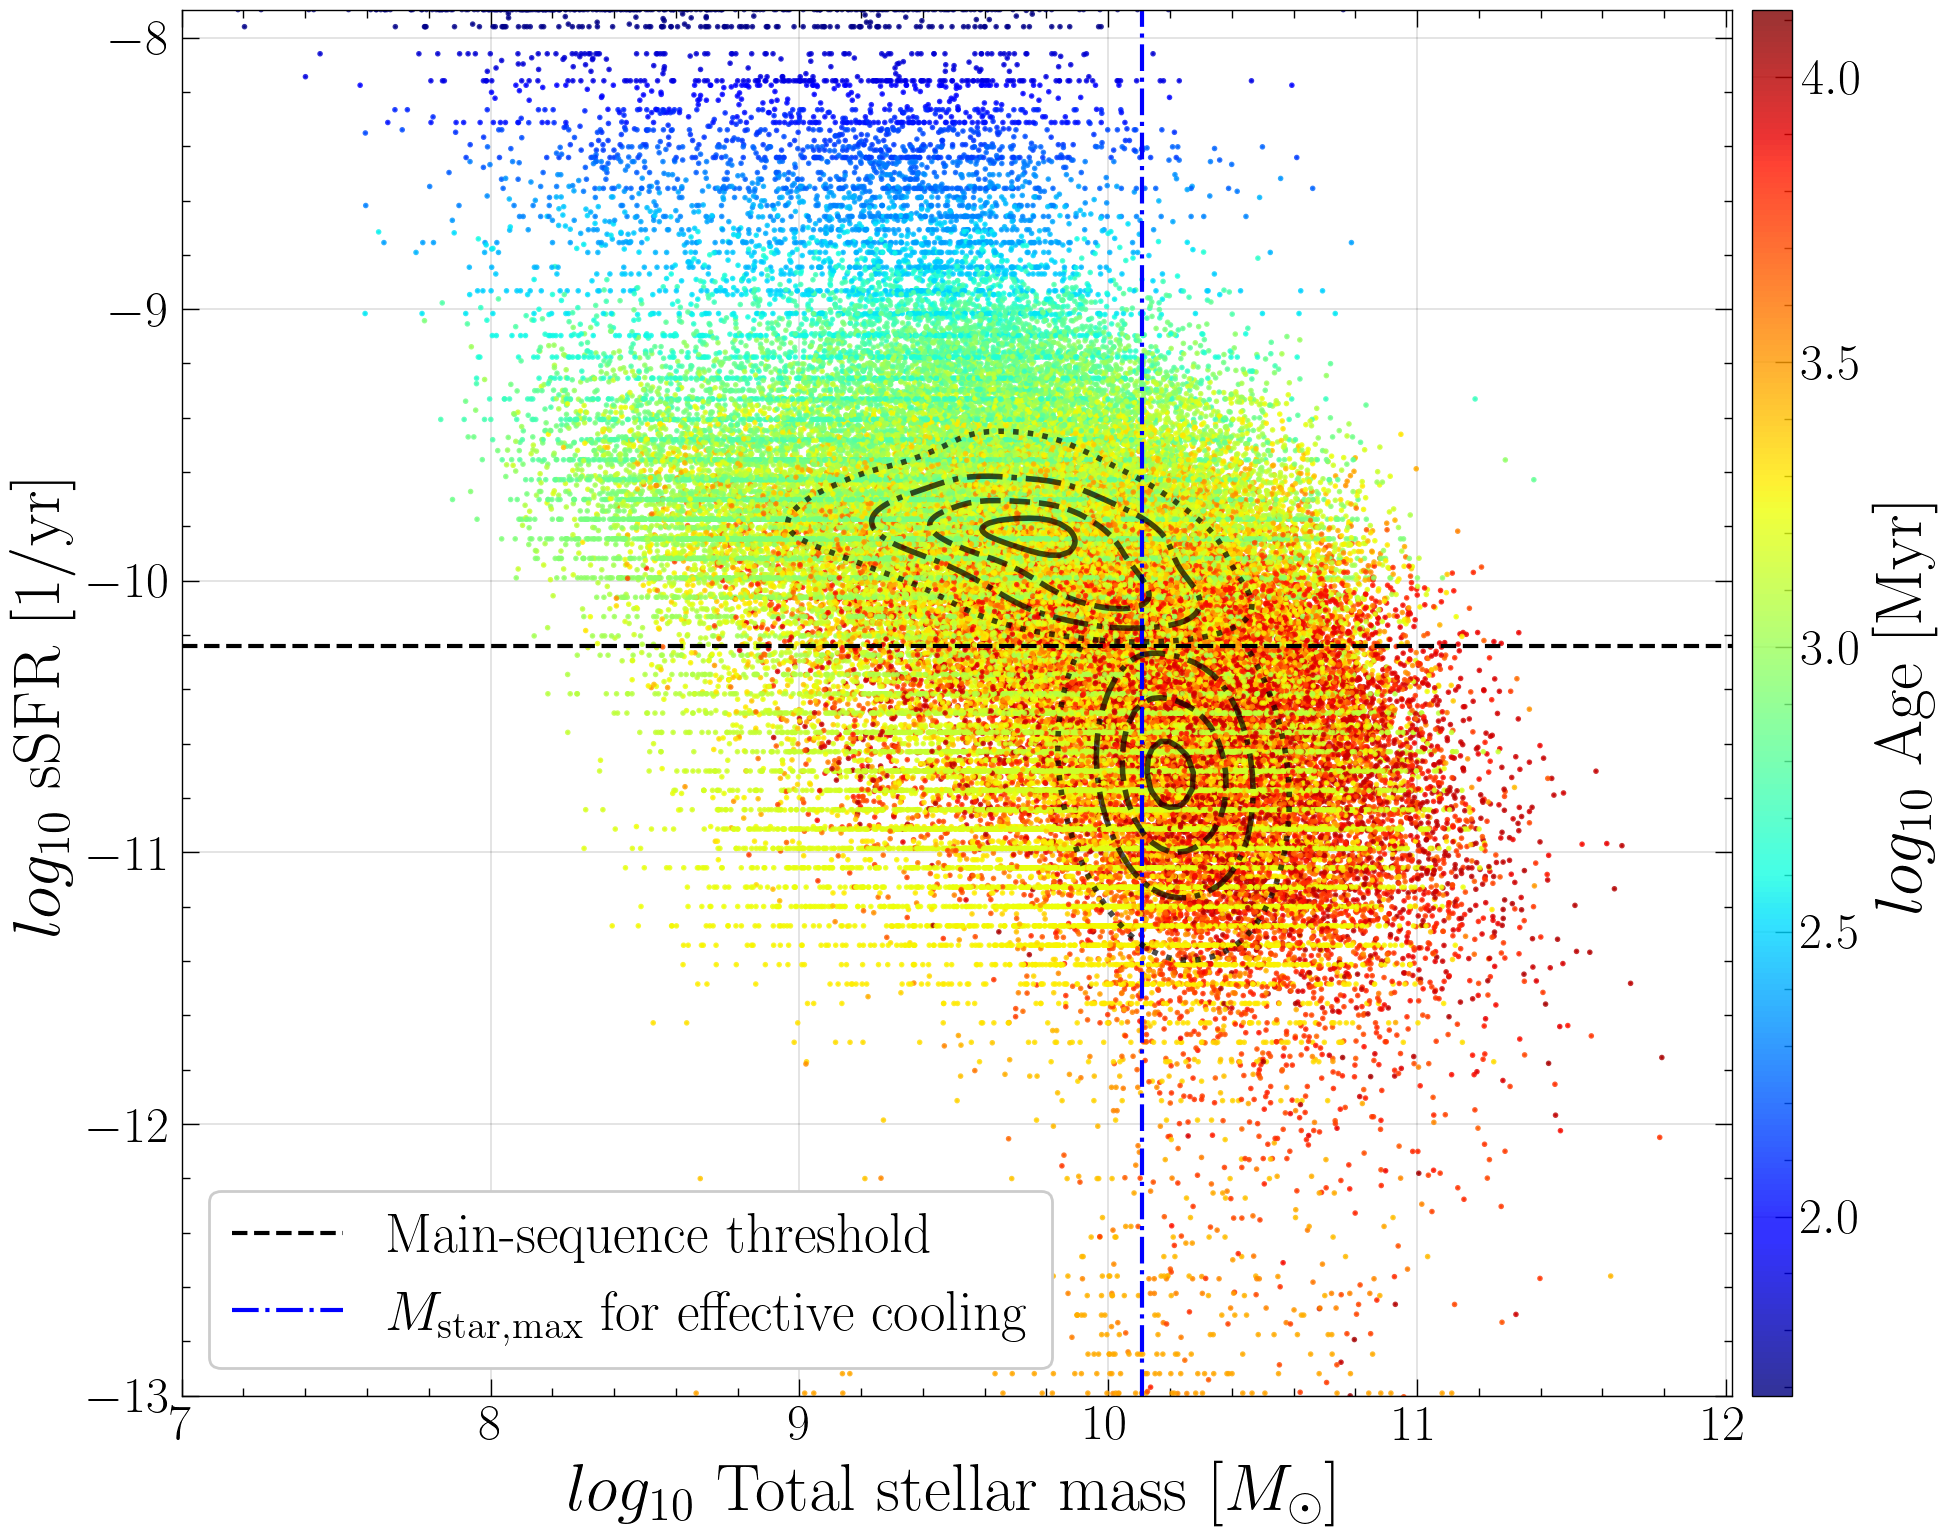
\includegraphics[width=0.84\columnwidth]{mass_sSFR_age.png}
    \caption{2D scatterplot of sSFR versus $M_{\text{star}}$ for our dataset, where the color is proportional to the age. The black dashed line separates the main sequence from passive galaxies. The blue dashdot line indicates $M_{\text{star,max}}$.The 25, 50, 75, and 95\% contours of both populations are shown.}
    \label{fig:mass_sSFR_age}
\end{figure}
We would like to derive a mathematical relation between the sSFR and $M_\text{star}$. Since the raw material for star formation is gas, we expect the SFR to be proportional to the amount of available gas, i.e., SFR$\propto M_\text{gas}^\alpha$, where the proportionality constant must have the dimensions of inverse time. We assume the linear relation originally found by \citet{Kennicutt_1998}:
\begin{equation}
    \text{SFR}\left(M_\text{gas}\right) \simeq \dfrac{\epsilon}{\tau_\text{dyn}} M_\text{gas} \doteq \epsilon' M_\text{gas},
	\label{eq:SFR_vs_gasmas}
\end{equation}
where $\epsilon \simeq 0.02$ is an efficiency parameter and $\tau_\text{dyn}$ is the dynamical time, which is given by:
\begin{equation}
    \tau_\text{dyn} = 2 \times 10^7 \text{yr} \left(\dfrac{R_{1\slash2}}{4\text{kpc}}\right) \left(\dfrac{v_\text{circ}}{200\text{km s}^{-1}}\right)^{-1}.
	\label{eq:t_dynamical}
\end{equation}
However, for simplicity we assume $\tau_\text{dyn} = 2 \times 10^7 \text{yr}$, because it has only a mild impact on the result.

In general, the time evolution of $M_\text{gas}$ can be described by:
\begin{equation}
    \dfrac{dM_\text{gas}(t)}{dt} \, = \, \dot{M}_\text{gas}^\text{in}(t) - \dot{M}_\text{gas}^\text{out}(t) - \left(1-R\right)\text{SFR}(t),
	\label{eq:dmgas_dt_old}
\end{equation}
where $R$ is the fraction of gas that undergoes the star formation process, but then returns to the gas reservoir due to stellar winds and supernovae.
As mentioned in Sec.~\ref{sec:introduction}, the gas outflow depends on a series of processes, but we only consider the most important: Type IIA supernovae. Their contribution can be simply written as:
\begin{equation}
    \dot{M}_\text{gas}^\text{out}(t) \, \simeq \, \eta\text{SFR}(t),
	\label{eq:mgas_outflow}
\end{equation}
where $\eta$ is the supernovae feedback parameter, that, in general, depends on time. Therefore, eq.~\ref{eq:dmgas_dt_old} becomes:
\begin{equation}
    \dfrac{dM_\text{gas}(t)}{dt} \, = \, \dot{M}_\text{gas}^\text{in}(t) - \left(1+\eta-R\right) \dfrac{\epsilon}{\tau_\text{dyn}} M_\text{gas}.
	\label{eq:dmgas_dt}
\end{equation}

Describing gas inflow is a little more complicated, as it depends on $M_\text{halo}$. In general, we can write:
\begin{equation}
    \dot{M}_\text{gas}^\text{in}(t) = \xi \, \dot{M}_\text{halo,\rm gas}^\text{in}(t) = \xi \, f_\text{gas} \, \dot{M}_\text{halo}^\text{in}(t),
	\label{eq:mgas_inflow}
\end{equation}
where we can assume $f_\text{gas}=0.15$ and $\xi \in [0,1]$ is a function related to the cooling efficiency discussed in Sec.~\ref{sec:introduction}. The simplest possible form for $\xi$ is a step-function:
{\fontsize{7.9pt}{7.9pt}\begin{equation}
    \xi_\text{step} =
    \begin{cases}
        0 \:\:\:\: \text{If} \: \tau_\text{cool} > \tau_\text{free-fall} \: , \: \text{i.e.} \: , \: M_{\text{halo}} \notin \left( M_{\text{halo,min}} \, , \, M_{\text{halo,max}} \right)\\
        1 \:\:\:\: \text{If} \: \tau_\text{cool} < \tau_\text{free-fall} \: , \: \text{i.e.} \: , \: M_{\text{halo}} \in \left( M_{\text{halo,min}} \, , \, M_{\text{halo,max}} \right)
    \end{cases}
	\label{eq:xi_step}
\end{equation}}

$\dot{M}_\text{halo}^\text{in}(t)$ is still unknown to us, but we can assume a relation obtained from the \textbf{Millenium Simulation} \citep{McBride_2009}:
{\fontsize{7.9pt}{7.9pt}\begin{equation}
    \dot{M}_\text{halo}^\text{in}(z) = 42 M_{\odot} \text{yr}^{-1} \left(\dfrac{M_\text{halo}}{10^{12}M_{\odot}}\right)^{1.127} (1+1.17z) \sqrt{(1+z)^3 \Omega_m + \Omega_\Lambda},
	\label{eq:mcbride}
\end{equation}}
where we can assume $\Omega_m=0.3$ and $\Omega_\Lambda=0.7$.
There is still an unknown quantity, $M_\text{halo}$. We can estimate it by numerically inverting the empirical relation found by \citet{Moster_2012}:
\begin{equation}
    M_\text{star} \left(M_\text{halo}\right) = 2N M_\text{halo} \left[\left(\dfrac{M_\text{halo}}{M_1}\right)^{-\beta} + \left(\dfrac{M_\text{halo}}{M_1}\right)^\gamma\right]^{-1},
	\label{eq:moster}
\end{equation}
where $N$, $\beta$, $\gamma$, and $M_1$ are coefficients that can be found in the original paper and that depend on redshift (we assume $z_{\text{mean}} \simeq 0.054$). We can use this relation to transform eq.~\ref{eq:halo_mass_minmax} into an efficient-cooling condition on $M_\text{star}$:
\begin{equation}
    M_\text{star} \in \left( M_\text{star,min}=10^{4.3} M_\odot \, , \, M_\text{star,max}=10^{10.1} M_\odot \right).
	\label{eq:star_mass_minmax}
\end{equation}
As shown in Fig.~\ref{fig:mass_sSFR_age}, most passive galaxies exceed $M_\text{star,max}$, and therefore, we expect them to have $\dot{M}_\text{gas}^\text{in} \approx 0$.
Moreover, we can see that passive galaxies are, on average, much older than star-forming ones. This suggests that the former may have already depleted their most massive stars, which die in powerful supernovae capable of ejecting gas out of the galaxy (i.e., $\eta \approx 0$). For these reasons, we can approximate the passive galaxies with a closed-box model, in which there is no exchange of gas between the galaxy and its halo. On the other hand, star-forming galaxies should be modeled with an open-box model, as we expect them to both accrete and eject gas. In the next sections, we will try to describe the two populations using one model for each, ideally merging into a single model with a sharp transition at $M_\text{star,max}$.


%%%%%%%%%%%%%%%%%%%%%%%%%%%%%%%%%%%%%%%%%%%%%%%%%%

\subsection{Open-box model at equilibrium for star-forming galaxies}\label{sec:open_box}
We can solve eq.~\ref{eq:dmgas_dt} analytically in three special cases: whether one of the two RHS terms is negligible with respect to the other, or when they are equal. In this last case, $M_\text{gas}$ is constant over time, and therefore this is an equilibrium solution. Since we want to describe star-forming galaxies with a model in which both accretion and ejection of gas are relevant, we consider the equilibrium case. From eq.~\ref{eq:dmgas_dt}, we get:
{\fontsize{7.9pt}{7.9pt}\begin{equation}
    M^\text{eq}_\text{gas}(t) = \dfrac{\dot{M}_\text{gas}^\text{in}(t)}{(1+\eta-R)\epsilon'} \: \Rightarrow \: sSFR^\text{eq}\left(M_{\text{star}}\right) = \dfrac{\dot{M}_\text{gas}^\text{in}\left(M_{\text{star}}\right)}{1+\eta-R} \, \dfrac{1}{M_\text{star}},
	\label{eq:openbox_equilibrium}
\end{equation}}
where $\dot{M}_\text{gas}^\text{in}\left(M_{\text{star}}\right)$ is given by \cref{eq:mgas_inflow,eq:xi_step,eq:mcbride,eq:moster}, with $z_{\text{mean}} \simeq 0.054$, while $\eta$ and $R$ are free parameters of the model. Our result is represented by the red line in Fig.~\ref{fig:openbox_and_closedbox}. We set $\eta=0.9$ and $R=0.4$ to get the model as close as possible to the median of the star-forming galaxies, represented by the black solid line.

\begin{figure}\centering
	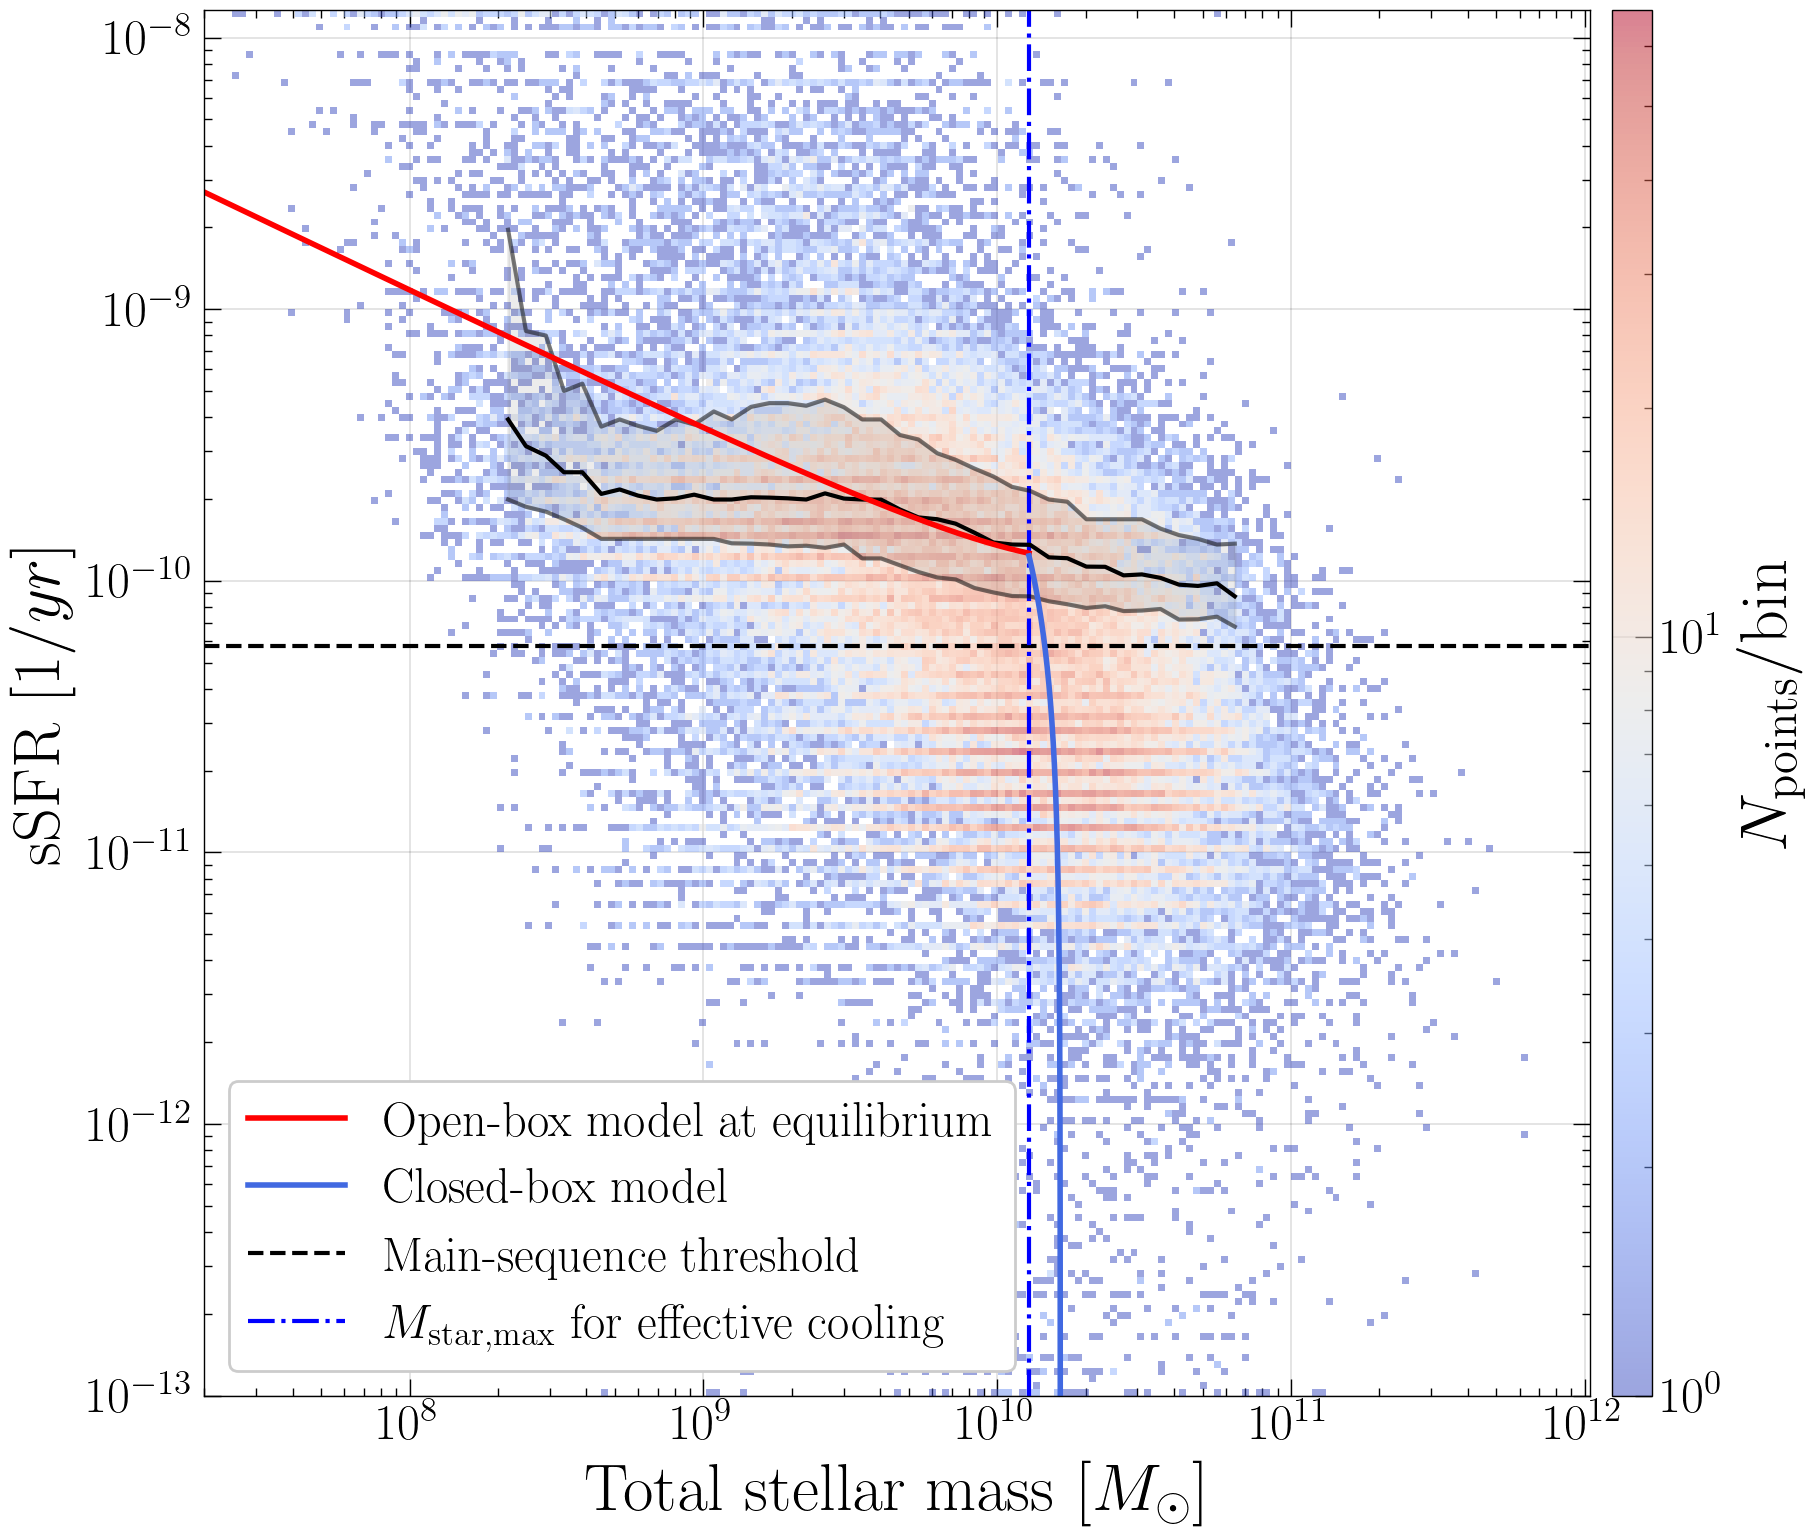
\includegraphics[width=0.9\columnwidth]{openbox_and_closedbox.png}
    \caption{2D histogram of sSFR versus $M_{\text{star}}$ for our dataset. The black dashed line separates the main sequence from passive galaxies. The black solid line is the median of the main sequence. The blue dashdot line indicates $M_{\text{star,max}}$. The red solid line is the open-box model at equilibrium. The blue solid line is the closed-box model.}
    \label{fig:openbox_and_closedbox}
\end{figure}
%%%%%%%%%%%%%%%%%%%%%%%%%%%%%%%%%%%%%%%%%%%%%%%%%%

\subsection{Closed-box model for passive galaxies}\label{sec:closed_box}
Closed-box model means setting $\dot{M}_\text{gas}^\text{in}=0$ and $\eta=0$ in eq.~\ref{eq:dmgas_dt}, which then becomes trivial:
\begin{equation}
    M_\text{gas}(t) = M_\text{gas}(t_0)\exp{[-(1-R)\epsilon' (t-t_0)]},
	\label{eq:mgas_closedbox}
\end{equation}
where $t_0$ is the time at which $M_{\text{star}}$ exceeds $M_\text{star,max}$ and, in our approximation, the closed-box model becomes valid. We can compute the SFR from eq.~\ref{eq:SFR_vs_gasmas} and integrate it, from $t_0$ to $t$, to obtain $M_{\text{star}}$:
\begin{equation}
    M_\text{star}(t) = M_\text{star}(t_0) + \dfrac{M_\text{gas}(t_0)}{1-R}\left{1-\exp{\left[-(1-R)\epsilon' (t-t_0)\right]}\right}.
	\label{eq:mstar_closedbox}
\end{equation}

\subsection{Numerical integration}\label{sec:numerical_integration}
\begin{figure}\centering
	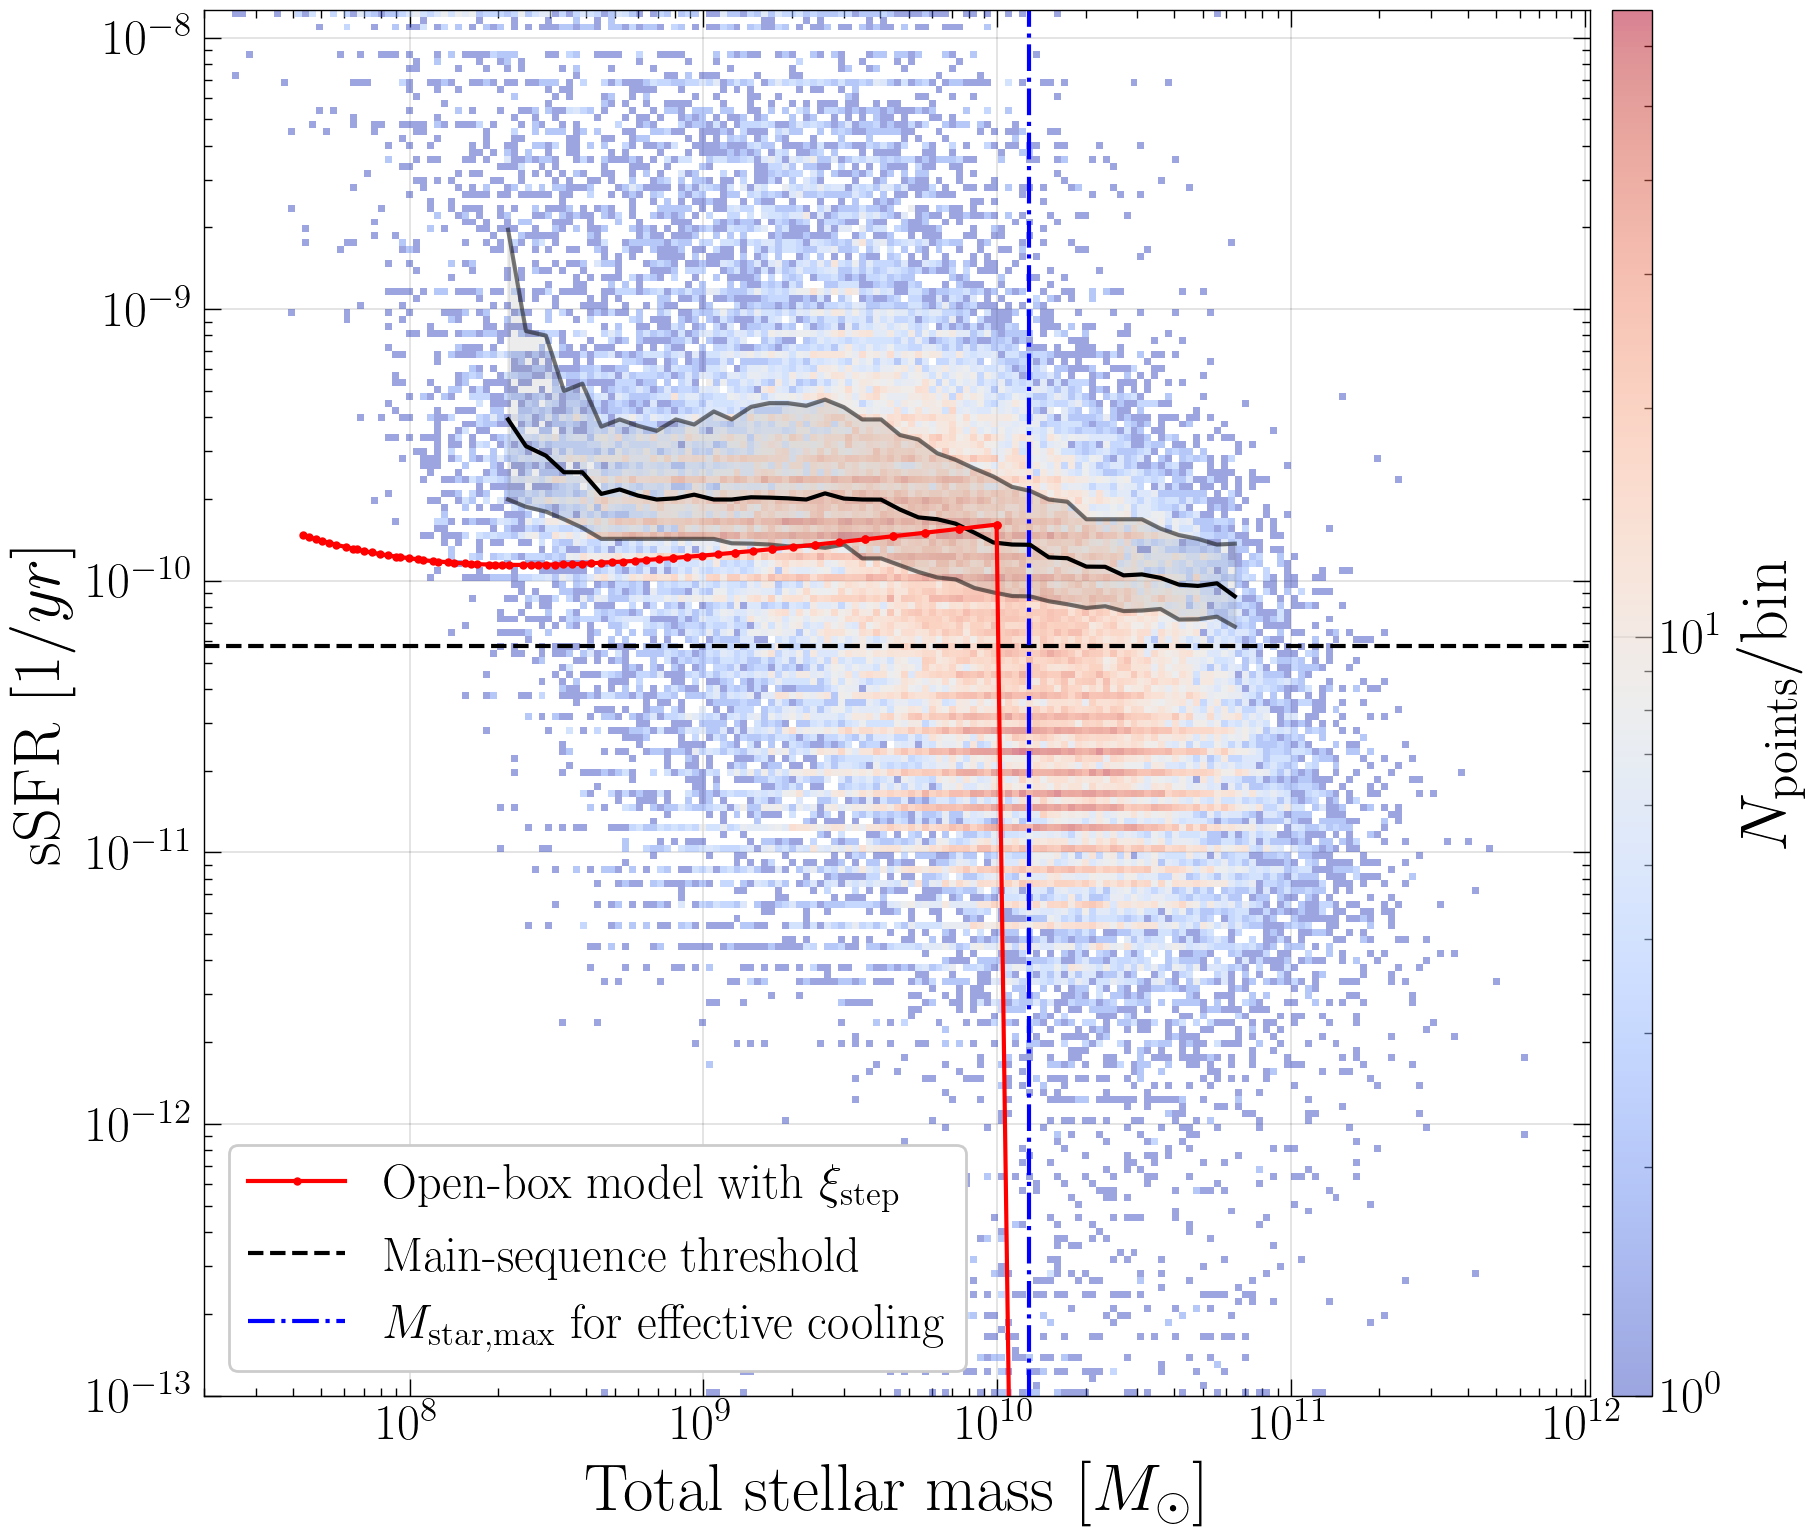
\includegraphics[width=0.9\columnwidth]{openbox_step.png}
    \caption{2D histogram of sSFR versus $M_{\text{star}}$ for our dataset. The black dashed line separates the main sequence from passive galaxies. The black solid line is the median of the main sequence. The blue dashdot line indicates $M_{\text{star,max}}$. The red solid line is the numerical open-box model with $\xi_\text{step}$.}
    \label{fig:openbox_step}
\end{figure}

\begin{figure}\centering
	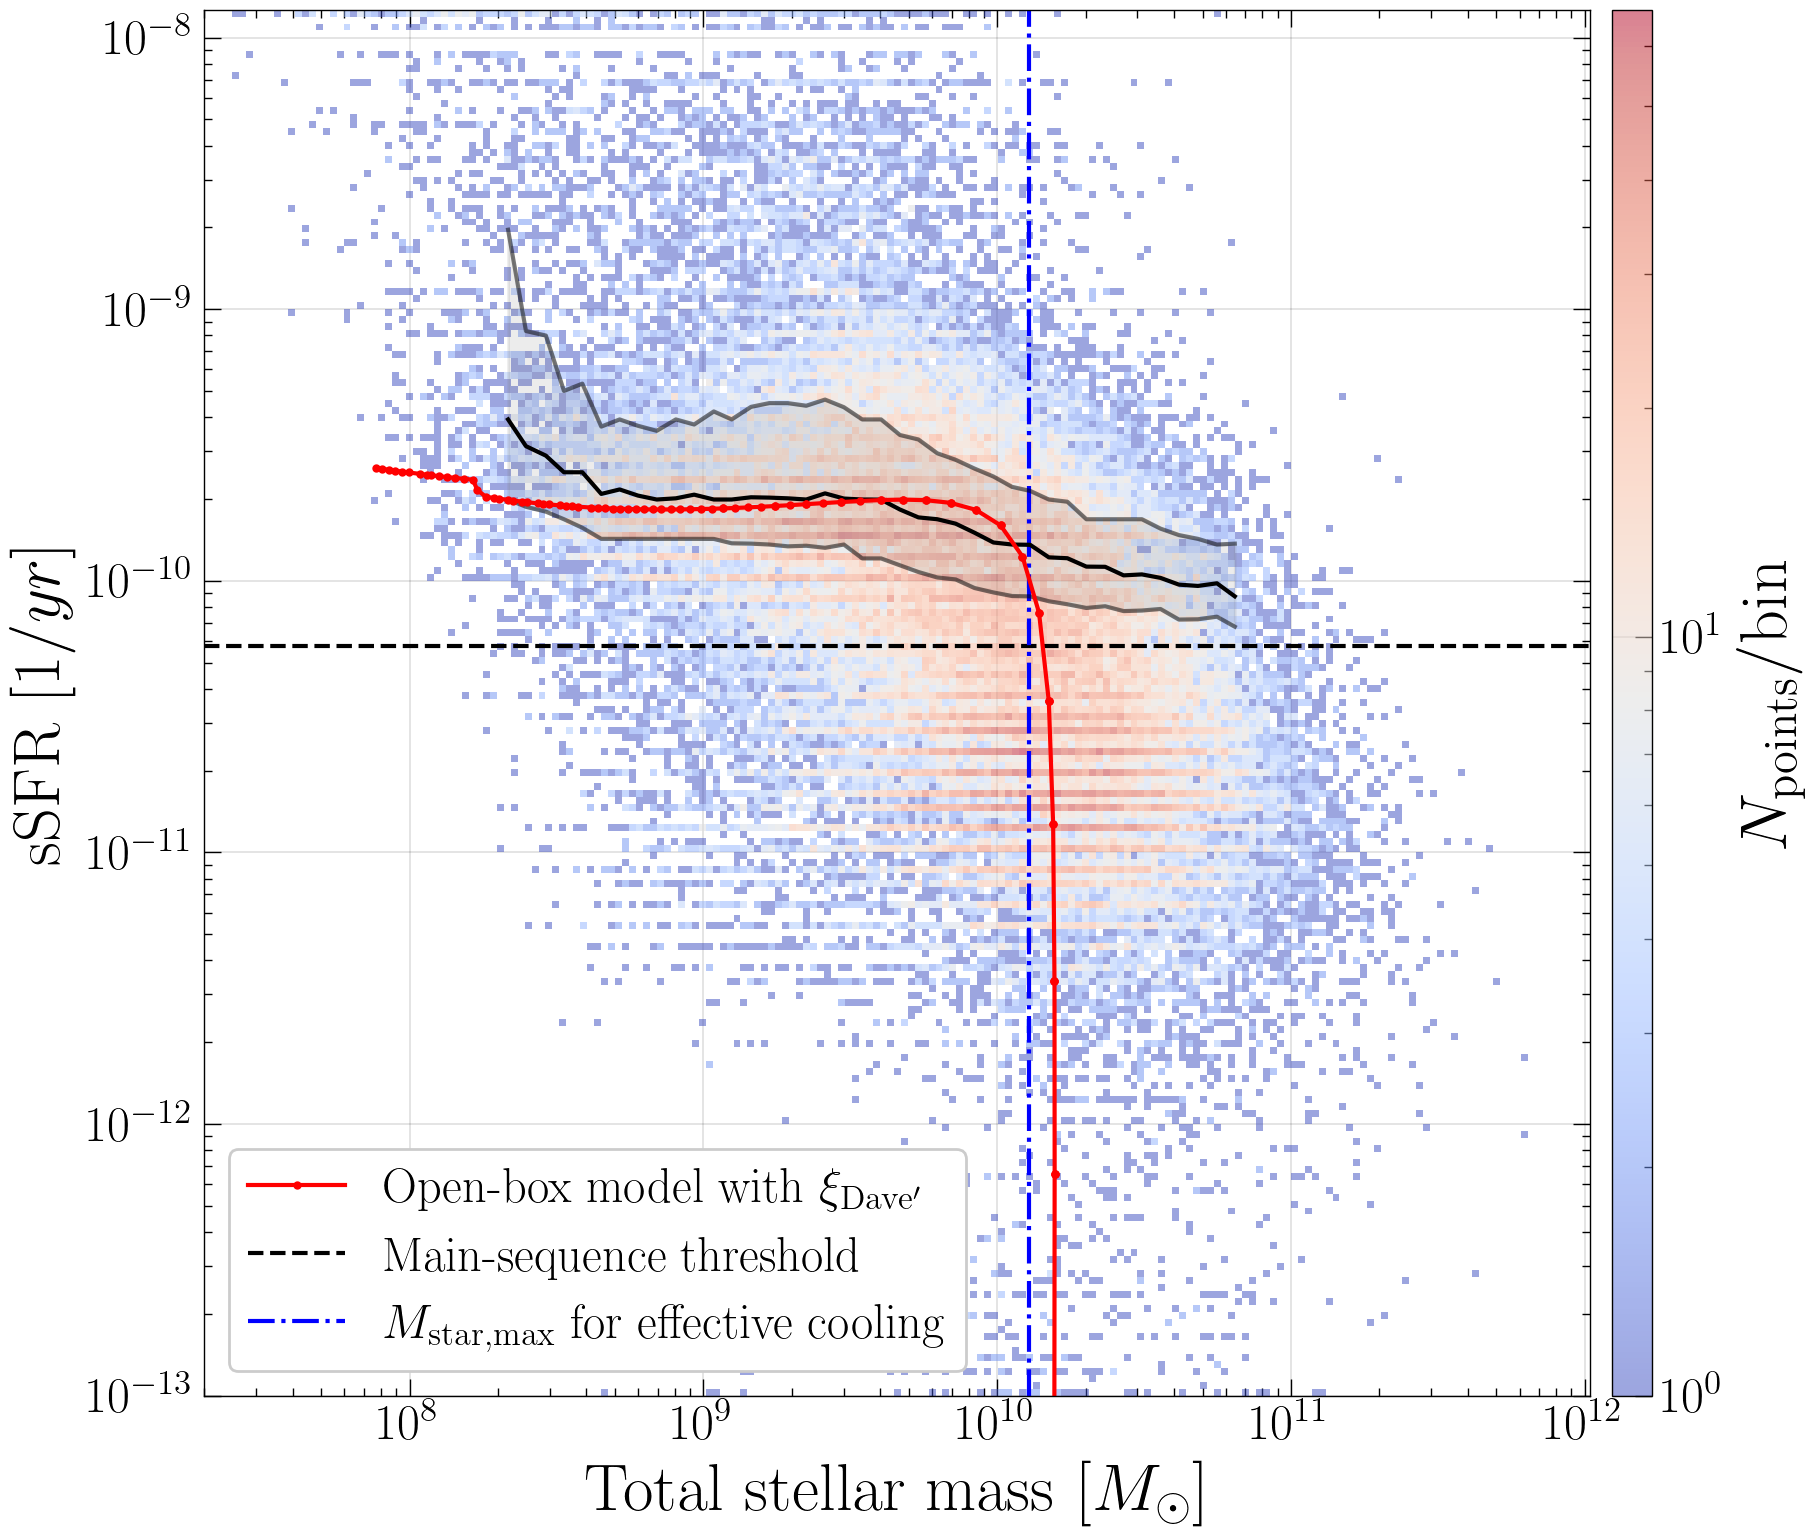
\includegraphics[width=0.9\columnwidth]{openbox_dave.png}
    \caption{2D histogram of sSFR versus $M_{\text{star}}$ for our dataset. The black dashed line separates the main sequence from passive galaxies. The black solid line is the median of the main sequence. The blue dashdot line indicates $M_{\text{star,max}}$. The red solid line is the numerical open-box model with $\xi_\text{Davé}$.}
    \label{fig:openbox_dave}
\end{figure}
%%%%%%%%%%%%%%%%%%%%%%%%%%%%%%%%%%%%%%%%%%%%%%%%%%



\section{Discussion}\label{sec:discussion}

%%%%%%%%%%%%%%%%%%%%%%%%%%%%%%%%%%%%%%%%%%%%%%%%%%



\section{Summary}\label{sec:summary}

%%%%%%%%%%%%%%%%%%%%%%%%%%%%%%%%%%%%%%%%%%%%%%%%%%%%%%%%%%%%%%%%%%%%%%%%%%%%%%%%%%%%%%%%%%%%%%%%%%%%




%%%%%%%%%%%%%%%%%%%% REFERENCES %%%%%%%%%%%%%%%%%%%%%%%%%%%%%%%%%%%%%%%%%%%%%%%%%%%%%%%%%%%%%%%%%%%%
% The best way to enter references is to use BibTeX:
\bibliographystyle{mnras}
\bibliography{bibliography} 
%%%%%%%%%%%%%%%%%%%%%%%%%%%%%%%%%%%%%%%%%%%%%%%%%%%%%%%%%%%%%%%%%%%%%%%%%%%%%%%%%%%%%%%%%%%%%%%%%%%%


% Don't change these lines
\label{lastpage}
\end{document}
